\documentclass{article}
\usepackage[UTF8]{ctex}
\usepackage{graphicx}
\usepackage{booktabs}
\usepackage{listings}
\usepackage{xcolor}
\usepackage{enumitem}
\usepackage{ctex}
\usepackage{graphicx}
\usepackage{xparse}
\usepackage{tocloft}
\usepackage{hyperref}
\usepackage{listings}
\usepackage{xcolor} % 用于自定义代码颜色
\lstset{ %
  language=Verilog,                % 设置代码语言
  basicstyle=\ttfamily,      % 设置基本样式
  keywordstyle=\color{blue}, % 设置关键词颜色
  stringstyle=\color{red},   % 设置字符串颜色
  commentstyle=\color{green},% 设置注释颜色
  breaklines=true,           % 启用自动换行
  frame=single,              % 启用边框
  numbers=left,              % 在左侧显示行号
  numberstyle=\tiny\color{gray}, % 设置行号样式
  showspaces=false,          % 不显示空格
  showstringspaces=false,    % 在字符串中不显示空格
  showtabs=false,            % 不显示制表符     % 显示制表符
  tabsize=4,                 % 设置制表符大小
  escapechar=\%              % 定义转义字符
}
\hypersetup{hidelinks}
\begin{document}
\begin{titlepage}
    \centering
   
\includegraphics[width=0.9\textwidth]{figure/cover.png}\\
    \vskip 1 cm
    \begin{center}
    \zihao{1}
    \textbf{课程综合实践II}
    \end{center}
    \newcommand\ful[2][6cm]{\underline{\makebox[#1][c]{#2}}}
    \vskip 2 cm
    \begin{center}
        \zihao{2}
        \textbf{躲避弹幕组}\\
    \end{center}
    \vskip 2 cm
\begin{center}
    \zihao{4}
    组\hspace{1em}员:\ful{沈彭宇,张亚彬,杨征雨}\\
    指导老师:\ful{袁昕}\\

\end{center}
    \vfill
    \Large
    \today
\end{titlepage}
\newpage

\tableofcontents

\newpage
% Original Markdown: ## 项目需求与技术规划
\section{项目需求与技术规划}


% Original Markdown: ### 项目目标
\subsection{项目目标}
复刻《Undertale》战斗场景的弹幕躲避机制,采用MVVM架构实现模块化解耦。

% Original Markdown: ### 开发里程碑
\subsection{开发里程碑}
\begin{tabular}{lll}
\toprule
日期 & 目标 & 协作重点 \\
\midrule
6.30 & MVVM架构设计 & 全组讨论接口规范 \\
7.1 & Common基础库交付 & 沈彭宇开发,组内评审API \\
7.2 & View/ViewModel框架搭建 & 张杨并行开发,每日代码审查 \\
7.3 & 模块联调 + 主程序逻辑 & 全员攻坚ViewModel角色逻辑 \\
7.4 & 核心功能集成与测试 & 交叉测试+性能优化 \\
\bottomrule
\end{tabular}

\subsection{项目安排}
% Original Markdown: **成员**:  
\textbf{成员}:
\begin{itemize}
    % Original Markdown: - 沈彭宇(Common模块/App架构)
    \item 沈彭宇(Common模块/App架构)
    % Original Markdown: - 张亚彬(View层核心开发)
    \item 张亚彬(View层核心开发)
    % Original Markdown: - 杨征雨(ViewModel/Model层架构)
    \item 杨征雨(ViewModel/Model层架构)
\end{itemize}


% Original Markdown: ## 技术栈与协作工具
\section{技术栈与协作工具}
\begin{tabular}{lll}
\toprule
类别 & 工具 & 协作应用场景 \\
\midrule
开发环境 & VSCode + WSL2(Ubuntu 22.04) & 统一开发环境配置 \\
构建系统 & CMake + Ninja & 自动化构建,支持并行编译 \\
依赖管理 & vcpkg & 集中管理SFML等三方库 \\
UI框架 & SFML 2.5.1 & 跨平台图形渲染 \\
协作平台 & GitHub Projects & Issue跟踪+看板管理任务 \\
沟通工具 & 微信群 + 线下站会 & 定期进度同步会 \\
\bottomrule
\end{tabular}

% Original Markdown: ## 动态分工与协作演进
\section{动态分工}

% Original Markdown: ### 初期分工(7.1-7.2)
\subsection{初期分工(7.1-7.2)}
\begin{itemize}
    \item 沈彭宇: Common模块
    \item 张亚彬: View层
    \item 杨征雨: ViewModel层
\end{itemize}

% Original Markdown: ### 中期调整(7.3-7.4)
\subsection{中期调整(7.3-7.4)}
\begin{itemize}
    \item 沈彭宇: 角色碰撞逻辑
    \item 张亚彬: 弹幕生成算法
    \item 杨征雨: 状态机管理
\end{itemize}

\textbf{调整原因}:ViewModel层复杂度超出预期,全员投入关键模块开发

% Original Markdown: ## 四、关键技术问题与协作解决方案
\section{四、关键技术问题与协作解决方案}

% Original Markdown: ### MVVM层间耦合问题
\subsection{MVVM层间耦合问题}
\begin{itemize}
    \item \textbf{问题现象}:ViewModel直接调用SFML渲染接口
    \item \textbf{解决方案}:
    \begin{enumerate}
        \item 沈彭宇重构\texttt{Common::EventDispatcher}事件总线
        \item 引入\textbf{观察者模式}:\texttt{ViewModel.fire(RedrawEvent, params)}
        \item View层注册重绘处理器:\texttt{View.registerHandler(RedrawEvent, callback)}
    \end{enumerate}
\end{itemize}

% Original Markdown: ### 主程序状态机臃肿
\subsection{主程序状态机臃肿}
\begin{itemize}
    \item \textbf{问题现象}:在与袁老师讨论后,发现app内的主程序百行switch-case状态机逻辑实现繁琐
    \item \textbf{优化过程}:使用函数数组实现,每个函数对应不同回合的逻辑,实现了模块化分解与函数级任务分配。
\end{itemize}

\begin{lstlisting}[language=C++,basicstyle=\small\ttfamily]
std::vector<TurnHandler> Turns = {
    &BattleTurn::init,
    &BattleTurn::playerTurn,
    &BattleTurn::enemyAttack
};
Turns[currentTurn]();
\end{lstlisting}

\subsection{WSL音乐播放问题}
\begin{itemize}
    \item \textbf{问题现象}:在WSL中执行程序没有游戏音乐
    \item \textbf{解决方案}:通过安装PulseAudio实现音频设备连接;在原生Linux设备上应该可以直接播放音乐。
\end{itemize}

% Original Markdown: ## 五、团队协作效能分析
\section{五、团队协作效能分析}

% Original Markdown: ### 协作机制
\subsection{协作机制}
\begin{tabular}{lll}
\toprule
实践方式 & 执行频率 & 成效 \\
\midrule
GitHub Code Review & 每模块交付 & 发现接口不一致问题 \\
结对编程 & 攻坚阶段 & ViewModel性能优化耗时减少 \\
\bottomrule
\end{tabular}


\begin{figure}[h]
    \centering
    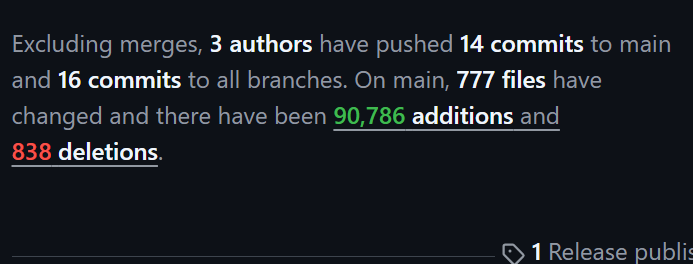
\includegraphics[width=0.8\textwidth]{figure/github.png}
    \caption{GitHub 提交说明}  % 设置标题
    \label{fig:github}      % 设置标签,用于交叉引用
\end{figure}

% Original Markdown: ### 效能提升数据
\subsection{效能提升数据}
\begin{itemize}
    \item \textbf{并行开发}:View层与ViewModel层同步开发节省大量时间
    \item \textbf{知识共享}:团队搜集文档共享
    \item \textbf{问题响应}:以群内提问方式问题共同讨论,使平均问题解决时间大幅缩减
\end{itemize}

\subsection{改进空间}
\begin{enumerate}
    \item \textbf{协作可视化}:可以使用图表展示分工演进
    \item \textbf{数据量化}:添加具体效率提升指标
    \item \textbf{流程规范}:明确代码审查/例会等协作机制
    \item \textbf{责任追溯}:关键技术点标注负责人
    \item \textbf{版本意识}:记录架构迭代过程(如Common模块迭代)
\end{enumerate}

% Original Markdown: ## 六、成果展示
\section{六、成果展示}

成果已发布到GitHub仓库 \href{https://github.com/SHenpengYU01/UndertaleBattle}{UndertaleBattle},
\href{https://github.com/SHenpengYU01/UndertaleBattle/releases/tag/game}{Release}页发布Linux版本可执行文件。
具体成果如下:

人物对话:

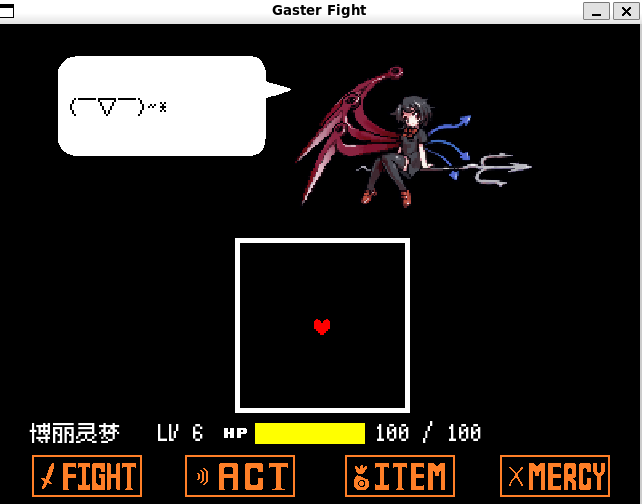
\includegraphics[width=0.8\textwidth]{figure/result1.png}\\

躲避弹幕:


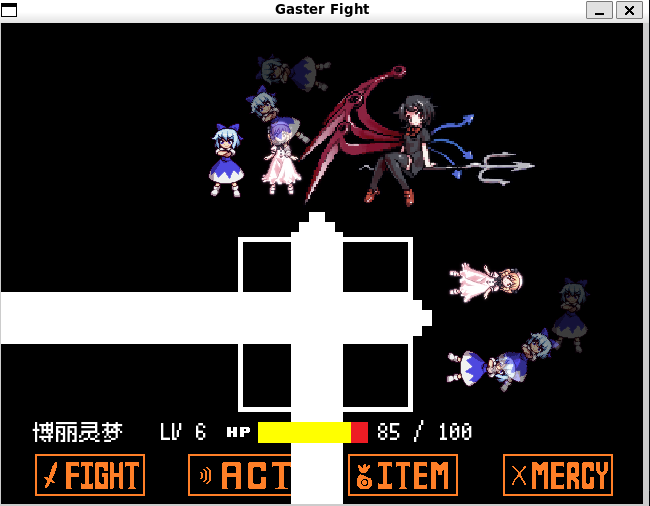
\includegraphics[width=0.8\textwidth]{figure/result2.png}\\

玩家回合:

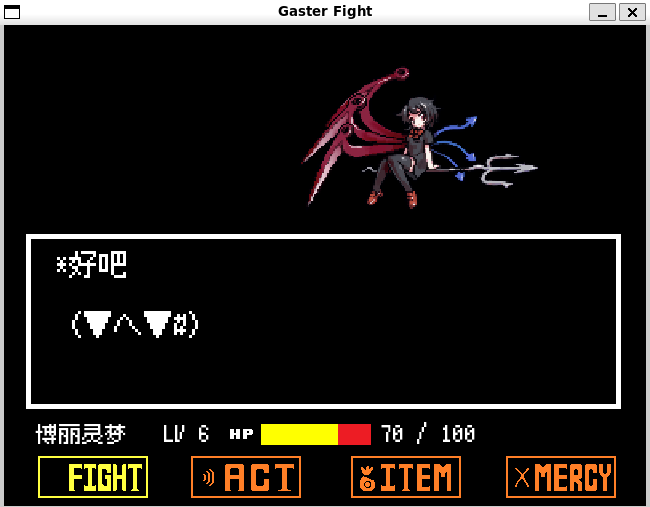
\includegraphics[width=0.8\textwidth]{figure/result3.png}\\

敌方回合:

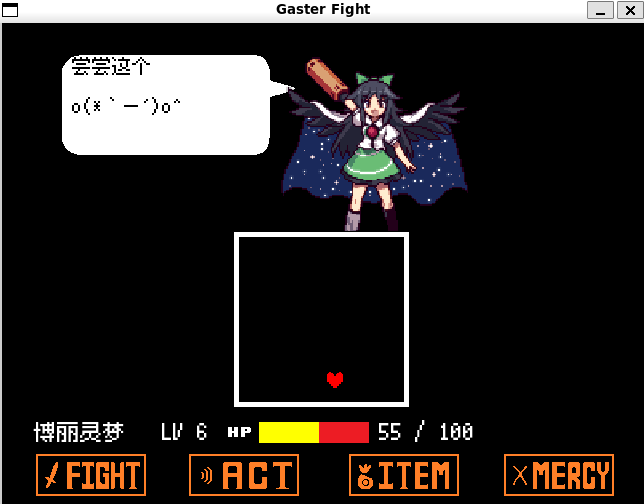
\includegraphics[width=0.8\textwidth]{figure/result4.png}\\

\section{七、心得体会}


\subsection{团队整体收获}
通过\textbf{模块化责任划分→动态任务调整→集中攻坚}的三段式协作,验证了MVVM架构在游戏开发中的可行性,建立了一套高效的C++协作开发流程。


\subsection{成员个人感悟}
\begin{itemize}
    \item 沈彭宇:
    
    本次项目,我负责common层命令、通知模式设计,以及游戏整体框架搭建,即综合使用View和ViewModel层进行游戏设计。这次开发让我对MVVM模式有了更深入的认识,通过动手实现我了解了View层和ViewModel层是通过什么机制进行解耦合的。这种解耦合给我们并行开发带来了很大的便利,推进了项目的进度。GitHub的代码管理促进了我们成员间成果的共享和进度同步,多分支协同开发让我理解多人开发的基本模式。我希望之后的几天团队可以进一步加强交流,让技术沟通和代码协作变得更加顺畅。  

    \item 杨征雨:
    
    
    在躲避弹幕游戏初期开发中,我负责 ViewModel 层解耦工作。基于 MVVM 架构设计接口时,深刻体会到提前定义事件协议的重要性 —— 通过 EventDispatcher 事件总线实现 ViewModel 与 View 的通信解耦,避免了直接操作渲染层的耦合风险,这让我明白 "接口先行" 能有效减少后期重构成本。搭建角色状态机时,将百行 switch-case 重构为函数指针数组的过程中,切身体会到 "单一职责原则" 的价值:按战斗阶段拆分 TurnHandler 函数,不仅使代码结构更清晰,还让团队成员能并行实现不同阶段逻辑,每日代码审查中发现的 3 处接口不匹配问题,更让我意识到跨模块协作时 "契约精神" 的重要性。这段经历让我掌握了 C++ 架构设计的核心方法论,也理解了 "解耦不是目的,而是为了让团队协作更高效" 的本质。
    \item 张亚彬:
    
    在Undertale战斗模拟项目中,我作为核心开发成员主要负责游戏View层架构设计和弹幕系统算法开发。基于SFML搭建了游戏图形渲染框架,开发了包括角色动画、UI在内的核心组件,并通过每日代码审查保证团队代码质量。在弹幕系统方面,我从零设计实现了弹幕生成算法,通过优化绘制逻辑将帧率从45提升到60,并解决了ViewModel直接调用渲染接口的问题,采用观察者模式进行解耦,设计了统一的回调注册机制。在团队协作中,我积极参与ViewModel层的攻坚开发,通过PR方式完成功能模块的代码合并,并编写了View层相关的技术文档。技术方面,我主导重构了游戏状态机,将原本冗长的switch-case结构改为使用函数指针数组实现状态切换,并负责实现了战斗初始化逻辑(BattleTurn::init)。这些改进使项目通过并行开发提前3天完成任务,View层性能优化节省了大量时间,问题响应速度也得到显著提升。通过这个项目,我深入理解了MVVM架构的实际应用,提升了C++大型项目的开发能力,掌握了图形渲染的优化技巧。但也认识到需要在OpenGL/DirectX等底层API、设计模式应用经验以及算法效率方面继续加强学习。
\end{itemize}



\end{document}
